
%************************************************
\chapter{Evolución de codificadores JPEG}\label{ch:resultados_evolucion}
%************************************************

% ============================================================
\section{Introducción a Cómputo Evolutivo}
% ============================================================

El \gls{Cómputo Evolutivo} es una rama de la Inteligencia Artificial que se define
por los tipos de algoritmos en los que se enfoca. Son algoritmos que utilizan
el concepto de la selección natural para resolver problemas de cómputo. Son
problemas de optimización en el sentido matemático. Es decir, se concentran en
encontrar un máximo local o un mínimo local utilizando heurísticas.


% ============================================================
\section{Algoritmos Evolutivos}
% ============================================================

Las características que los Algoritmos Evolutivos tienen en común son:

\begin{itemize}
\item Definen una población
\item Definen una función de aptitud.
\item Utilizan mutación y reproducción junto con la función de aptitud para
mejorar la población a lo largo de varias generaciones.
\end{itemize}

Aunque comparten la misma idea, se definen distintos tipos de algoritmos con
respecto a la manera en que concretizan estas características.

\begin{itemize}
\item La \emph{Programación Genética} \cite{GenProg} tiene conjuntos de
programas como su población. Su función de aptitud es la capacidad de un
programa para resolver cierto problema. Los programas se representan como
árboles de sintaxis, y de esta manera se define la mutación y reproducción como
operaciones en árboles.
\item La \emph{Programación Evolutiva} es similar a la Programación Genética
pero lo que se evoluciona son los parámetros de los programas, no su
estructura.
\item Los \emph{Algoritmos Genéticos} definen genotipos y su correspondiente
función de aptitud que evalúa los fenotipos respectivos. Es decir, se opera
sobre el cromosoma pero se evalúa el organismo.

El algoritmo desarrollado entra dentro de la clasificación de Algoritmo
Genético. El fenotipo es una tabla de cuantificación y el genotipo es un
codificador \gls{JPEG} que usa esa tabla.

\end{itemize}

% ============================================================
\section{Método para la evolución de codificadores JPEG}
% ============================================================

\subsection{Población}

Se inicializa una población de tablas. En el conjunto se incluye la tabla que
tiene todos sus coeficientes iguales a 1, denominada \emph{\gls{tabla
unitaria}}. La tabla unitaria es la que obtiene la mejor calidad posible pero
resulta en menor compresión. El resto del conjunto se llena de tablas con
valores aleatorios entre 1 y 64.

La función de aptitud requiere de un punto de referencia. Antes de iniciar la
evolución, se comprime la imagen con la tabla unitaria, dándonos un punto de
referencia para la calidad óptima y para el máximo tamaño.

\subsection{Selección}

La calidad de la compresión se determina haciendo una decodificación y
comparando la imagen resultante con la original píxel por píxel. Las
diferencias absolutas se suman. No se utiliza MSE (Error cuadrático medio) por
la enorme cantidad de pixeles y la sensibilidad del algoritmo a errores de
precisión. En lugar de implementar un decodificador JPEG, se incluye un paso de
decodificación en la función principal de procesamiento de bloques. Los
detalles de este proceso se explican en el capítulo \ref{ch:implementacion}.

El tamaño es más fácil de comparar que la calidad de la imagen. Tan solo es
necesario ver cuántos bits pesa la imagen resultante comparada con el tamaño
máximo que se obtiene de la tabla unitaria.

Tenemos dos garantías. Cualquier tabla de cuantificación comparada con la
unitaria va a resultar en mayor compresión y en menor calidad, siempre y cuando
la tabla a comparar no sea en sí una tabla unitaria.

Sea $T$ una tabla de nuestra población y sea $T_0$ la tabla unitaria.

Definimos nuestra función de aptitud como:

\begin{equation}
f(T) = \frac{e(T)}{e(T_0)} + \alpha \Big(1 + \frac{s(T)}{s(T_0)}\Big)
\end{equation}\label{eq:fitness}

\dots donde $e(T)$ es el error de compresión y $s(T)$ es el tamaño de la
imagen. $\alpha$ es una constante que se usa para ajustar la importancia que le
damos al tamaño sobre la compresión o vice versa.

Nótese que los dos términos se afectan mutuamente. Una tabla que tiene mayor
compresión va a tener un mayor error, y una tabla con menor compresión resulta
en una imagen de mayor calidad. En otras palabras, cuando el primer término
disminuye, el segundo crece.  Cuando el segundo término crece, el primero
disminuye.

Nuestra meta es encontrar $T$ tal que $f(T)$ es mínima. La relación entre los
dos términos permite que el algoritmo converja.

El primer término es siempre mayor o igual a $1$. A la fracción del segundo
término se le suma 1 porque el valor de $\frac{s(T)}{s(T_0)} \in (0, 1]$. Esto
es puramente una una conveniencia para facilitar la búsqueda de un valor de
$\alpha$ adecuado.

El valor de $\alpha$ controla el proceso de minimización. Mientras mayor sea
$\alpha$, más peso de aptitud tiene el tamaño de la imagen. El algoritmo tiende
a 'preferir' minimizar el error contra el tamaño después de cierto umbral de
$\alpha > 1$. Para valores de $\alpha \leq 1$, se producen imágenes de muy mala
calidad.

Habiendo probado varios valores distintos, se encontró que un valor de $\alpha
= 2$ resulta en imágenes que son indistinguibles de las originales, con un alto
nivel de compresión.


\subsection {Mutación y Reproducción}

Cada generación, sobreviven las dos mejores tablas. El resto se parte en dos.

Con las pruebas que se hicieron, se encontró que con el método de cruza y de
mutación que se está utilizando, la taza más efectiva es dividir 50\% de la
población para ser mutada, y 50\% para ser cruzada. En la mayoría de los casos
esto resultó en una convergencia más rápida con mejores valores al evaluar la
función de aptitud.

El proceso de mutación es como sigue: Cada entrada de la tabla tiene una
probabilidad de $\frac{1}{64}$ de mutar. Cuando una entrada $e$ muta, lo hace
sumando a su valor original $e_{nueva} = e_{vieja} + x $ donde $x \in [-4, 4]$
con distribución de probabilidad uniforme.

El proceso de reproducción siempre ocurre entre las dos tablas ganadoras. Padre
A y Padre B.  La tabla hijo es el resultado de, para cada entrada, escoger una
entrada de Padre A o de Padre B. La elección es un tiro de moneda. Para alguno
de los dos padres, cada entrada tiene un $50\%$ de probabilidad de venir de él.

\subsection {Fin de la evolución}

El algoritmo decide terminar cuando sucede una de dos cosas:

\begin{itemize}
\item El número de generaciones llega a 100
\item Dado el individuo más apto de generación previa $x_p$ y el de la generación actual, $x_0$, sucede cuatro veces consecutivas que $f(x_p) - f(x_0) \leq 0.0001$, donde $f$ es la función de aptitud \ref{eq:fitness}.
\end{itemize}

Al final de la evolución, se toma la tabla ganadora y se usa como entrada para
el codificador \gls{JPEG}.

\section{Codificador Evolutivo}

El nombre del proyecto final es \emph{gp\_encoder}. Consta de un algoritmo
evolutivo que utiliza a DummyJPEG para su función de aptitud y a TinyJPEG
para codificar la imagen resultante.

% ============================================================
\section{Conjuntos de prueba} \label{sec:testset}
% ============================================================

El proyecto está dividido en tres partes: TinyJPEG: la implementación de JPEG
con compresión \emph{baseline} basada en la especificación \cite{jpeg-spec};
DummyJPEG: la versión modificada de JPEG que sirve para tener una función de
selección paralelizable, que tiene implementaciones paralelas para CPU y GPU; y
finalmente, el proyecto completo, que consta de un algoritmo evolutivo descrito
en el capítulo \ref{ch:evolucion}, que utiliza DummyJPEG en su función de
aptitud y emite el resultado usando TinyJPEG.

La biblioteca TinyJPEG, a partir de ser lanzada como código libre, consiguió
una base de usuarios. Actualmente hay gente usándola en aplicaciones que van
desde tareas escolares hasta proyectos de investigación \cite{humblebrag}.
Durante un año se han encontrado distintos errores de implementación que no
aparecieron con los decodificadores de prueba que se utilizaron durante su
desarrollo. La exposición al ``mundo real'' que ha tenido la biblioteca ha sido
de gran ayuda para dar un cierto nivel de confianza de que la implementación es
correcta.

El proyecto \emph{gp\_encoder} se ha beneficiado directamente de la exposición
de TinyJPEG. DummyJPEG es un clon directo, y cualquier error de TinyJPEG que
pudo haber afectado a DummyJPEG fue corregido. La única porción del trabajo que
no ha tenido la ventaja de ser probado en el ``mundo real'' es la implementación
OpenCL de DummyJPEG. Sin embargo, no ha dado problemas para las pruebas que se
han hecho durante el desarrollo de gp\_encoder.

Para el propósito de mostrar resultados en este documento, se utilizan cuatro
imágenes de ejemplo. Más adelante mostramos las imágenes y damos las razones
por las cuales fueron elegidas.

Uno de los puntos débiles de JPEG es que no es bueno lidiando con
discontinuidades. Una queja común es que al comprimir imágenes de caricatura,
JPEG tiene problemas con los delineados, como se muestra en la figura
\ref{fig:gibbs}. A esto se le conoce como el Fenómeno de Gibbs \cite{gibbs}, y
puede aparecer en la literatura de procesamiento de señales como \emph{ringing
artifacts}. El fenómeno describe la manera en que se comportan las Series de
Fourier cuando se encuentran con un salto discontinuo. Esto es exactamente lo
que sucede cuando vemos ``delineados'' en caricaturas que se comportan mal
cuando se codifican con JPEG. La DCT es un caso particular de la transformada
de Fourier, como se menciona en el capitulo \ref{ch:jpeg_desc}.

\begin{figure}[b]
    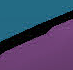
\includegraphics[width=1.0\textwidth]{gibbs}
    \caption{Fenómeno de Gibbs en una imagen JPEG}
    \label{fig:gibbs}
\end{figure}

La imagen ``Klay'' (figura \ref{fig:ref-klay}) es una captura de un pantalla de
un juego cuyo estilo presenta muchos saltos discontinuos.

La imagen ``Diego'' (figura \ref{fig:ref-diego}) es una fotografía que presenta
mucho ruido, gracias al fondo de mármol.

La imagen ``Ghost'' es una captura de pantalla del Anime \emph{Ghost in the
Shell}. Es un punto medio entre el ruído de ``Diego'' y el estilo caricaturesco
de ``Klay''

Finalmente, la imagen ``Pluto'' (figura \ref{fig:ref-pluto}) es una fotografía
publicada por NASA cuando la sonda \emph{New Horizons} pasó cerca de Plutón en
Septiembre de 2015. La imagen tiene una resolución de $8000\times8000$ y su
principal propósito es mostrar cómo se comportan los diferentes componentes del
proyecto cuando se presenta una carga de trabajo grande relativamente a las
demás imágenes.

\begin{figure}[b]
    \includegraphics[width=1.0\textwidth]{ref_klay}
    \caption{Klay}
    \label{fig:ref-klay}
\end{figure}

\begin{figure}[b]
    \includegraphics[width=1.0\textwidth]{ref_diego}
    \caption{Diego}
    \label{fig:ref-diego}
\end{figure}

\begin{figure}[b]
    \includegraphics[width=1.0\textwidth]{ref_ghost}
    \caption{Ghost}
    \label{fig:ref-ghost}
\end{figure}

\begin{figure}[b]
    \includegraphics[width=1.0\textwidth]{ref_pluto}
    \caption{Pluto}
    \label{fig:ref-pluto}
\end{figure}

% ============================================================

% ============================================================
\section{Convergencia}
% ============================================================

Recordando la ecuación que usamos para nuestra función de aptitud:

\begin{equation}
f(T) = \frac{e(T)}{e(T_0)} + \alpha \Big(1 + \frac{s(T)}{s(T_0)}\Big)
\end{equation}\label{eq:fitness-repeated}

Se desea obtener la cota mínima.

Se sabe que $e(T_0)$ es siempre menor o igual a $e(T)$, ya que $T_0$ es la
tabla de cuantificación que consiste solo de valores 1, que denominamos
\emph{tabla unitaria}, que resulta en lo más cercano en JPEG con compresión
\emph{baseline} a una compresión sin pérdida. Por lo tanto, el primer parámetro
de la ecuación está en $[1, \infty)$.

De manera análoga, el tamaño de la imagen resultante al comprimir con la tabla
unitaria es el mayor posible. Entonces, el término $\frac{s(T)}{s(T_0)} \in (0,
1]$. Se encontró que un buen valor de $\alpha$ para conseguir imágenes de alta
calidad es 2. Por lo tanto, el segundo término de la ecuación $f(T)$ está en
$(2, 4]$

En base a esto, se concluye que para la función de aptitud, con una tabla de
cuantificación arbitraria, el mínimo valor posible es 3.

En esta sección se incluyen las gráficas de convergencia para la función de
aptitud al correr gp\_encoder con las cuatro imágenes de referencia:
\ref{img:plot-diego}, \ref{img:plot-ghost}, \ref{img:plot-klay}, \ref{img:plot-pluto}.

Todas las figuras mostradas están normalizadas a 50 generaciones con un rango
de evaluación de la función de aptitud entre 3.5 y 5. Se usa una gráfica de
línea para mostrar el valor de la función de aptitud para los individuos más
aptos y se utilizan puntos para los peores individuos de cada generación. Se
usan puntos porque comúnmente ocurre que en alguna generación, el individuo
menos apto tenga un valor de aptitud mucho mayor a 5. El caso común, sin
embargo, es que los individuos menos aptos también tienden a un punto de
convergencia mientras la evolución avanza.

Cabe notar que la gráfica para la imagen ``Pluto'' \ref{img:plot-pluto} muestra
que hubo una convergencia en un número de generaciones relativamente pequeño.
Para ver lo que pasaba, se cambió la tasa de mutación:cruza de 0.5 a 0.8,
resultando en la figura \ref{img:plot-pluto2}. Esto resulta en una gráfica
\emph{``escalonada"}, mostrando una evolución de 57 generaciones que produce
una tabla con valor de aptitud similar al del resultado original. Fue
consistente el encontrar que cualquier distribución distinta a 50/50 producía
peores resultados.

\begin{figure}[b]
    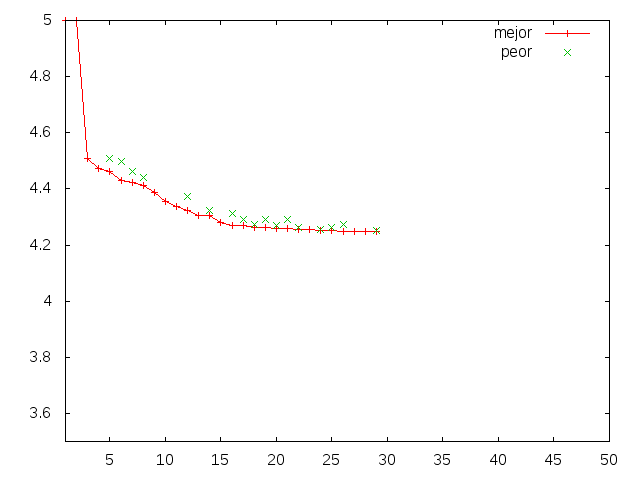
\includegraphics[width=1.0\textwidth]{plot_diego}
    \caption{Convergencia para imagen ``Diego"}
    \label{img:plot-diego}
\end{figure}

\begin{figure}[b]
    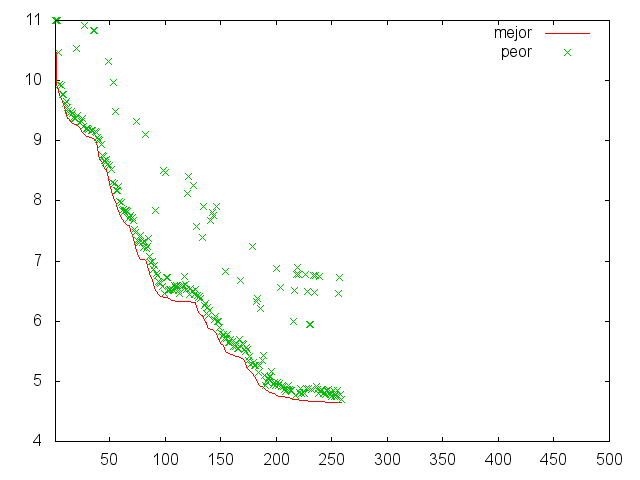
\includegraphics[width=1.0\textwidth]{plot_ghost}
    \caption{Convergencia para imagen ``Ghost"}
    \label{img:plot-ghost}
\end{figure}

\begin{figure}[b]
    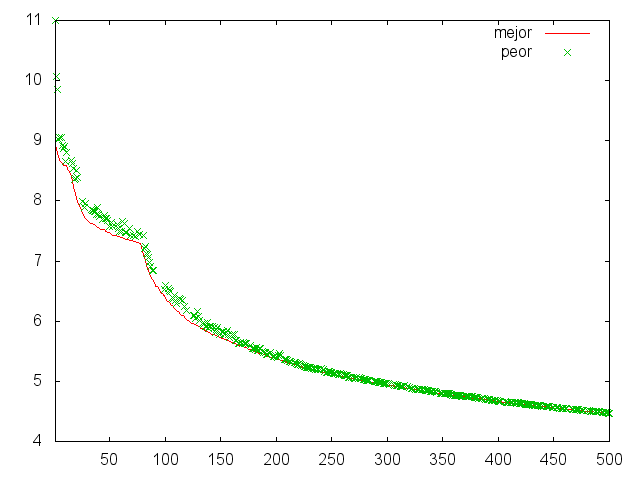
\includegraphics[width=1.0\textwidth]{plot_klay}
    \caption{Convergencia para imagen ``Klay"}
    \label{img:plot-klay}
\end{figure}

\begin{figure}[b]
    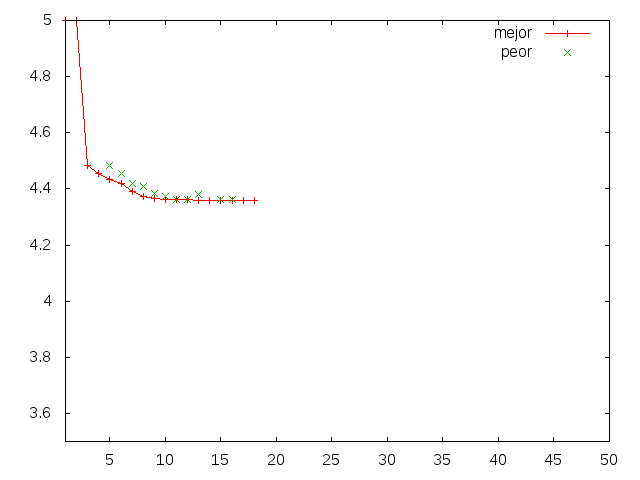
\includegraphics[width=1.0\textwidth]{plot_pluto}
    \caption{Convergencia para imagen ``Pluto"}
    \label{img:plot-pluto}
\end{figure}

\begin{figure}
    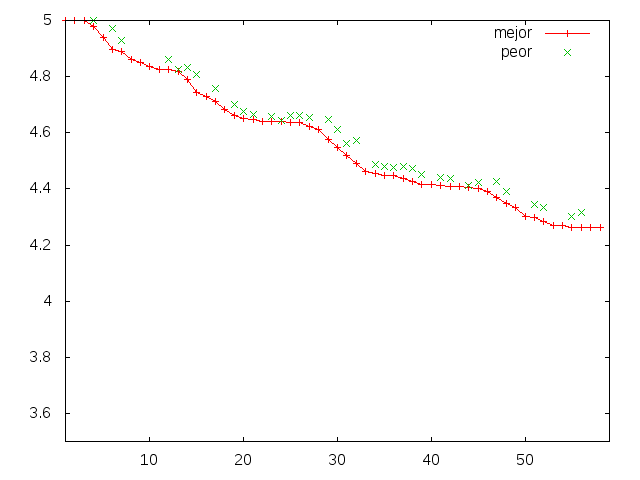
\includegraphics[width=1.0\textwidth]{plot_pluto_tweak}
    \caption{Convergencia para imagen Pluto con una tasa de mutación a cruza diferente}
    \label{img:plot-pluto2}
\end{figure}

% ============================================================
\section{Comparación de resultados}
% ============================================================

La tabla \ref{fig:perf_table} es una copia de la que se mostró en el capítulo
\ref{ch:implementacion}. Muestra el desempeño de gp\_encoder en sus
diferentes modalidades: CPU (single-thread y multi-thread) y GPU (OpenCL).

\begin{figure}[h!]
    \begin{tabular}{ |l c c c c r| }
        \hline
        Nombre &  Un Thread & Múltiples Threads & GPU & Speedup MT & Speedup GPU \\
        \hline
        Diego & 10.796s & 5.210s & 1.391s  & 2.072X & 7.76X \\
        Ghost & 13.706s & 6.607s & 1.760s  & 2.257X & 7.78X \\
        Klay & 40.526s & 22.279s & 4.785s  & 1.819X & 8.46X \\%, 4.65
        Plutón & 558.83s & 204.120s & 13.940s & 2.73X & 40.08X \\ % 14.64
        \hline
    \end{tabular}
    \caption{Tabla de desempeño para gp\_encoder}
    \label{fig:perf_table}
\end{figure}

El algoritmo evolutivo se desarrolló con el propósito de generar imágenes
indistinguibles de las originales pero con una buena tasa de compresión. En la
tabla \ref{fig:size-table} comparamos los tamaños de las imágenes de prueba
originales con su versión comprimida con la tabla de cuantificación
evolucionada y la compresión "media" de TinyJPEG, descrita en el capítulo
\ref{ch:implementacion}.

Con la excepción de la imagen de Plutón, gp\_encoder resulta en imágenes codificadas de menor tamaño.

Tanto con TinyJPEG en calidad media como con los resultados de gp\_encoder, todas las imágenes son indistinguibles de la original, excepto por Klay.

La imagen de Klay es interesante porque gp\_encoder consigue hacerla
indistinguible de la original, a diferencia de TinyJPEG, que falla a calidad
media. Encima de lograr esto, el nivel de compresión es 1.56X mejor. 419K de
TinyJPEG contra 268K de gp\_encoder. Esto sugiere que el algoritmo evolutivo
desarrollado en este proyecto es una estrategia viable para aplicaciones que
requieran usar JPEG incluso cuando el tipo de imágenes con las que se está
tratando no son ideales para el formato.

Para ilustrar la diferencia entre la imagen Klay comprimida con TinyJPEG y la
resultante de gp\_encoder, se incluye la imagen \ref{img:banding}, con TinyJPEG
a la izquierda y gp\_encoder a la derecha. A la izquierda puede observarse un
efecto de bandas de color más marcado que el que aparece en el lado derecho.
Cabe notar que las bandas de color del lado derecho también aparecen en la
imagen original, y son el resultado de no aplicar \emph{dithering} dentro del
motor del juego que produjo la imagen original.

\begin{figure}
    
\includegraphics[width=400pt, height=200pt]{banding}
    \caption{Izquierda: TinyJPEG. Derecha: gp\_encoder}
    \label{img:banding}
\end{figure}

Para finalizar, se incluye la tabla de cuantificación evolucionada para la
imagen Klay (figura \ref{fig:klay-table}). Vale la pena compararla con la tabla de
cuantificación de referencia \ref{fig:reference-table} para observar las
características poco intuitivas de la tabla generada por gp\_encoder, como la
relativa alta cantidad de coeficientes de valores bajos en las frecuencias
altas.


\begin{equation}
    \begin{matrix}
        1  &   8  &  1  & 20  &  1  & 16  & 38  & 12 \\
        37 &   59 &  44 &  21 &  18 &  14 &   4 &  11 \\
        23 &   54 &  49 &  33 &  42 &  15 &  27 &  45 \\
        53 &   43 &  32 &  34 &   6 &  28 &   6 &   4 \\
        4  &  63  & 39  & 10  & 15  &  2  &  1  &  4 \\
        10 &    1 &  17 &  10 &  28 &   7 &   8 &  47 \\
        46 &   28 &   3 &  20 &   1 &  39 &   8 &  31 \\
        5  &  34  &  4  & 31  & 12  & 15  & 43  & 39
    \end{matrix}
    \label{fig:klay-table}
\end{equation}

\begin{figure}[h]
    \begin{tabular}{|l c c r|}
        \hline
        Nombre & Original & TinyJPEG & gp\_encoder \\
        \hline
        Diego & 2.3M & 355K & 328K \\
        Ghost & 2.6M & 562K & 366K \\
        Klay  & 9.1M & 419K & 268K \\
        Pluto & 192M & 26M & 31M  \\
        \hline
    \end{tabular}
    \caption{Tamaños de imagen original y con compresión}
    \label{fig:size-table}
\end{figure}


